%{
%Formål med afsnit:
%\begin{itemize}
%	\item Problematikken med heltal, herunder hvor tæt vi kommer
%		egentlig på $\varPhi$.
%	\item Hvordan forholder vores approksimation sig ifht. Markovs
%		fejlmargin?
%	\item Vurdering af præcision.
%	\item Fortælle om de hjælpemetoder vi vil få brug for.
%\end{itemize}


\subsection*{Hvordan deles billedet efter det gyldne snit}
Et et billedet befinder der sig 4 gyldne snit, 2 i det vertikale plan og
2 i det horisontale pland. plasseringen af de 4 snit udregnes i forhold
til udledningen i afsnitet om det gyldne snit, hvor konstanten $\varPhi
= 1.618$ bliver fundet. Den horisontale brede og vertikale højte bliver
divideret med $\varPhi$. Denne udregning giver to tal som er hvor mange
pixels fra kanten begge kanter, det gyldne snit skal tegnes f.eks ved et
billedet som er 4000 pixel brad, vil punktet ligge hved.

\begin{equation}
	4000/\varPhi = 4000*2/(\sqrt{5}+1) = 2472.13595 \approx 2472
\end{equation}

\begin{figure}[h]
	\begin{center}
		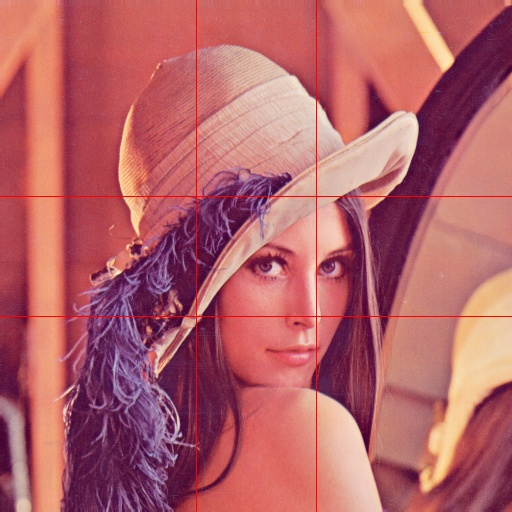
\includegraphics[scale=0.42,angle=0]{afsnit/vores_implementation/billeder/naiv_algoritme/Lenagolden}
	\end{center}
	\caption[]{Billedet som har indtegnet de fire gyldne snit}
	\label{f}
\end{figure}

\subsection*{Problematikken med helta}
Mange af de metoder som vi bruger til at udregne, position af det gyldne
snit eller størelsen af en margin, udregnes hved hjælp af brøkker.
Tilgendgel, er et billldet opbygget af pixels, Dette gør at vi må nød
til at tage aproximationer af udregningerne for at få dem tilbage til et
helt tal, men hvor meget af dataen er tabt, og hvor maget af
resultaterne kan man stole på.

\subsubsection*{Heltal i det gyldne snit}
Eksemplet med 4000 pixels ovenfor, approximere vi antal pixels ved at
rounde talet, dette gør at vi mister 0.13595 nøjagtighed, dette svare
til en misvisning af punktet på 0.00339875 $\%$ i forholdt til breden på
billedet. 

\begin{equation}
	0.13595/4000*100 = 0.00339875
\end{equation}

For at gøre det lidt mere generat, sætter vi den mistet nøjagtighed til
0.5, det er den max mistet nøjagtighed vi kan have, og sætter billedet
størelse til 500(dette er jeg ikke sikker på,) pixels, som er det miste
billedet vi har, dette giver en fejl margen på 0.1 $\%$. Dette resultat
befinder sig stadig meget lavt, og det kan konkluderes at, selv om vi
renger med en aproximation af det gyldne snit få vi stadig et resultat
som kan bruges.

\subsubsection{Heltal ved udregning af Margin}
En af vores mål ved denne opgave er at se om kunstner har tegnet
intrasante objektor ved opdelingen af billedet, ved 5/3 som snit, og
samme line det med det gyldne snit. Da disse 2 snit ligger meget tæt på
hinanden og vi gerne vil lave en sammenlining, er det viktigt at margin
for snittet ikke kryser hinanden. Dette vil endebære at de samme
objektor vil blive fundet af begge snit, og vil give et skævt billedet
af forskellen på de to snit.
hvis x betegner antale pixels i enden braden eller højden, og vil se
forskelen mellem 5/3 og $\Phi$, dividere vi x med snittet for at finde
dens plasering og substrahere dem fra hinanden.

\begin{equation}
	|\frac{x3}{5} - \frac{x2}{\sqrt{5}+1}| 
\end{equation}

Vi har taget den eqklidiske norm af formlen, da vi gerne ser at det
bliver et positivt andtale pixels som skelder de 2 snit. Vi har nu
fundet antal pixels mellem de to snit, og da vi gerne vil undgå at de 2
marginens ikke krysser hinanden, dividere vi med 2 og tager en floor på
helle funktionen.

\begin{equation}
	floor(\frac{|\frac{x3}{5} - \frac{x2}{\sqrt{5}+1}| }{2})
\end{equation}

Dette giver os et andtal af pixels som skilder de to snit. For at vise
hvor stort marginen egenlide kan være, bruger jeg denne formel på to
billeder, et som har svart til vores minste billedet, 500 pixels, og et
som svare til vores største billedet, 4000 pixels. Ved 500 pixels
bliver resultatet

\begin{equation}
	floor(\frac{|\frac{500*3}{5} - \frac{500*2}{\sqrt{5}+1}| }{2}) = 4
\end{equation}

Dette er en ok margin, lidt smådt, men vores test viser at det er
riglige til at finde godt ragioner i billedet.
Ved 4000 pixels giver det.

\begin{equation}
	floor(\frac{|\frac{4000*3}{5} - \frac{4000*2}{\sqrt{5}+1}| }{2}) = 36
\end{equation}
Som må siges at være mere end riglige.
% vim: set tw=72 spell spelllang=da:
